\documentclass[a4paper, 11pt]{article}
\usepackage[utf8]{inputenc}
\usepackage[T1]{fontenc}
\usepackage{lmodern}
\usepackage[german] {babel}
\usepackage[scaled]{helvet}
\renewcommand\familydefault{\sfdefault} 
\usepackage{lipsum}
\usepackage{cprotect}
\usepackage{fancyhdr}
\usepackage{amsmath}
\usepackage{amsfonts}
\usepackage{amssymb}
%\usepackage{environ}
%\usepackage{makeidx}
\usepackage{tikz}
%\usetikzlibrary{calc,matrix}
%\def\checkmark{\tikz\fill[scale=0.4] (0,.35)-- (.25,0)-- (1,.7)-- (.25,.15)-- cycle;} 
\usepackage{graphicx}
\usepackage{kpfonts}
\usepackage{tabularx}
\usepackage{multirow}
\usepackage{xcolor}
% TIMELINE
\newcommand\ytl[2]{
\parbox[b]{6em}{\hfill{\color{cyan}\bfseries\sffamily #1}~$\cdots\cdots$~}\makebox[0pt][c]{$\bullet$}\vrule\quad \parbox[c]{8.5cm}{\vspace{4pt}\color{black}\raggedright\sffamily #2.\\[5pt]}\\[-3pt]}
\usepackage{booktabs}
\usepackage{graphicx}
\usepackage{footnote}
\makesavenoteenv{figure}
\usepackage{epigraph}
\usepackage{listings}
\lstset{literate=% Allow for German characters in lstlistings.
{Ö}{{\"O}}1
{Ä}{{\"A}}1
{Ü}{{\"U}}1
{ß}{{\ss}}2
{ü}{{\"u}}1
{ä}{{\"a}}1
{ö}{{\"o}}1
}
\lstset{
    language=bash, %% Troque para PHP, C, Java, etc... bash é o padrão
    basicstyle=\ttfamily\small,
    numberstyle=\footnotesize,
    numbers=left,
    backgroundcolor=\color{gray!10},
    frame=single,
    tabsize=2,
    rulecolor=\color{black!30},
    title=\lstname,
    breaklines=true,
    breakatwhitespace=true,
    framextopmargin=2pt,
    framexbottommargin=2pt,
    extendedchars=false,
    inputencoding=utf8
}
\usepackage{hyperref}
\usepackage[
acronym,
nonumberlist,
toc,
nopostdot]{glossaries}
\usepackage[
maxbibnames=99,
backend=biber,
style=ieee,
sorting=ynt
]{biblatex}
\setcounter{biburllcpenalty}{7000}
\setcounter{biburlucpenalty}{8000}
\DeclareFieldFormat{journaltitle}{#1\isdot}
\DeclareFieldFormat[article]{citetitle}{#1}
\DeclareFieldFormat[article]{title}{#1}
\DeclareFieldFormat[report]{citetitle}{#1}
\DeclareFieldFormat[report]{title}{#1}
\DeclareFieldFormat[inproceedings]{citetitle}{#1}
\DeclareFieldFormat[inproceedings]{title}{#1}
\addbibresource{references.bib}
\usepackage{color}
\definecolor{dkgreen}{rgb}{0,0.6,0}
\definecolor{dkblue}{rgb}{0,0,0.4}
\definecolor{gray}{rgb}{0.5,0.5,0.5}
\definecolor{mauve}{rgb}{0.58,0,0.82}
\definecolor{darkerred}{rgb}{0.4,0,0}
\lstset{frame=tb,
    language=Java,
    aboveskip=3mm,
    belowskip=3mm,
    showstringspaces=false,
    columns=flexible,
    basicstyle={\small\ttfamily},
    numbers=none,
    numberstyle=\tiny\color{gray},
    keywordstyle=\color{blue},
    commentstyle=\color{dkgreen},
    stringstyle=\color{mauve},
    breaklines=true,
    breakatwhitespace=true,
    tabsize=3
}
\hypersetup{
    colorlinks = true,
    linkcolor=dkblue,
    filecolor=magenta,      
    urlcolor=cyan,
}
\renewcommand*{\glstextformat}[1]{\textcolor{darkerred}{#1}}
\usepackage[doublespacing]{setspace}
\usepackage{background}
\usepackage{lastpage}
\newcommand{\subautor}[1]{\begin{flushright}
    {\small\textit{#1}}    
\end{flushright}}
\backgroundsetup{contents={}}
\pagestyle{fancy}
\renewcommand{\headrulewidth}{0pt}% removes header line
\lhead{}
\rhead{}
\cfoot{\thepage}

\AtBeginDocument{\addtocontents{toc}{\protect\thispagestyle{empty}}}

\makeglossaries{}
\input{attachments/glossar-alex}
\newglossaryentry{g-abk}{
    name={Abkürzung},
    plural={Abkürzungen},
    description={
        Das ist nur ein Beispiel für einen Akronym und Glossareinträge.
    }
}

\input{attachments/glossar-miri}
\input{attachments/acronyms-alex}
\newglossaryentry{abk}{
    type=\acronymtype,
    name={Abk.},
    plural={Abkn.},
    description={\gls{g-abk}},
    first={Abkürzung (Abk.)\glsadd{g-abk}},
    firstplural={Abkürzungen (Abkn.)\glsadd{g-abk}},
}
\newglossaryentry{KI}{
	type=\acronymtype,
	name={KI},
    plural={KI},
    description={Künstliche Intelligenz},
    first={Künstliche Intelligenz (KI)},
    firstplural={Künstliche Intelligenzen (KI)},
}
\input{attachments/acronyms-miri}
\begin{document}
    \pagestyle{empty}
    \begin{titlepage}
    \begin{figure}
        \begin{flushright}
            
\includegraphics[scale=0.75]{images/INFLogo.png}
        \end{flushright}
    \end{figure}

    {\centering
    \vspace{1.5cm}
    {\Large Artefakt}\\

    \vspace{0.5cm}
    {\Large SAT}\\
    {\Large SoSe 2020}\\

    \vspace{1.0cm}
    \Large{\textbf{
            Kriterien für die Zulassung von medizinischen Produkten mit Künstlicher Intelligenz
          }
    }\\

    \vspace{1.0cm}
    \setstretch{0,8}
    {\small Alex Pollok}\\
    {\small 764359}\\
    {\small \href{mailto:alex_mark.pollok@student.reutlingen-university.de}{alex{\textunderscore}mark.pollok@student.reutlingen-university.de}}\\
    \vspace{0.5cm}
    {\small Evelyn Krebes}\\
    {\small 762780}\\
    {\small \href{mailto:evelyn_sophie.krebes@student.reutlingen-university.de}{evelyn{\textunderscore}sophie.krebes@student.reutlingen-university.de}}\\
    \vspace{0.5cm}
    {\small Miriam Lang}\\
    {\small 764532}\\
    {\small \href{mailto:miriam.lang@student.reutlingen-university.de}{miriam.lang@student.reutlingen-university.de}}\\

    \vspace{2.0cm}
    {\small Betreuer: Prof. Dr. rer. nat. Christian Kücherer\\}
    
	\backgroundsetup{
      scale=1,
      color=black,
      opacity=1,
      angle=0,
      position=current page.south,
      vshift=60pt,
      hshift=-210pt,
      contents={%
      \begin{minipage}{.18\textwidth}
      
\includegraphics[width=1000pt,height=70pt,keepaspectratio]{images/FHRTFooter.png}
      \end{minipage}%
      }    
    }
    }
\end{titlepage}

    \newpage
    \setstretch{1.0}
    {\centering
{\large Abstract (Evelyn)\\}
}
Künstliche Intelligenz (KI) ist ein immer größer werdender, stark wachsender Bereich in der Medizin.
Sie unterstützt, mit der Funktion des maschinellen Lernens,
unter anderem das Diagnostizieren von Krankheiten, die Entwicklung von Medikamenten,
das Personalisieren von Behandlungen und Verbesserungen von Genbearbeitung.
Damit die medizinischen KI-Produkte in der Medizin eingesetzt werden dürfen,
gibt es erforderliche Zulassungsverfahren und Vorgaben, die eingehalten werden müssen.
Welche Verfahren in Europa und den Vereinigten Staaten bisher bestehen,
wird in diesem Artikel zusammen mit den notwendigen Kriterien
für die Zulassung von medizinischen KI-Produkten erörtert.
Die Verwendung dieser Produkte, deren Vorteile,
Grenzen und weitere Lösungsansätze für die Zulassung sowie die Frage,
ob die bisher bestehenden Kriterien ausreichend sind,
werden hier mit einer Literaturanalyse untersucht.
Trotz bereits angepasster Zulassungsverfahren der medizinischen KI-Produkte,
zeigt sich,
dass weitere Anpassungen durch die regulierenden Behörden nötig sind.
        
    \newpage
    \hypertarget{contents}{}
    \tableofcontents

    \newpage
    \pagestyle{fancy}
    \setstretch{1.0}
    \section{Einführung \small{(Alex)}}\label{sec:introduction}
        In diesem Kapitel geben zuerst einen Überblick über den Kontext der Arbeit und weshalb die Zulassungskriterien für Medizinische Produkte mit Künstlicher Intelligenz eine genauere Untersuchung benötigen. Dann stellen wir die Ziele unserer Arbeit vor und wie wir unsere Forschungsfragen beantworten wollen. Zuletzt wird die Struktur der Arbeit kurz dargestellt.
		\subsection{Motivation, Kontext und Gegenstand}\label{sec:motivationcontext}
			\begin{itemize}
	\item Fokus der Arbeit auf Richtlinien und nicht Software Qualitätsmerkmale
\end{itemize}
		\subsection{Ziele}\label{sec:goals}
			Unsere Hauptforschungsfrage lautet "`Welche Probleme bestehen bei der Zulassung von medizinischen Produkten mit KI unterstützter Software?"'(FF1).
Der Fokus der Arbeit liegt auf den Zulassungsverfahren von medizinischen Produkten. Wir wollen die Zulassungsverfahren für medizinische Produkte untersuchen und prüfen ob sie auch für KI im medizinischem Bereich geeignet sind. Dazu müssen wir zuerst bestimmen welche Kriterien ein Medizinisches Produkt mit KI erfüllen sollte. Deshalb lautet die erste unserer Unterforschungsfragen "`Welche besonderen Kriterien sind für die Zulassung von KI in der Medizin notwendig?"'(FF2). 
Da wir mit unserer Arbeit prüfen wollen ob die Richtlinien für medizinische Produkte mit KI ausreichend sind müssen wir auch den aktuellen Stand der Verfahren untersuchen und was bisher getan wurde um die Richtlinien anzupassen. Deshalb stellten wir uns die Unterforschungsfrage "`Inwieweit gelten die aktuellen Richtlinien auch für Produkte mit KI?"'(FF3). Zuletzt wollen wir untersuchen ob der Einsatz von KI in der Medizin vorteilhaft für den Patienten ist und wie weit diese Vorteile reichen. Dazu formulierten wir als letzte Unterforschungsfrage "`Welche Vorteile bringen KI dem Patienten gegenüber und welche Grenzen haben diese Vorteile?"'(FF4).
			\subsubsection{Zentrale Fragestellung}\label{sec:questions}
				Unsere Hauptforschungsfrage lautet:
\begin{itemize}
\item Welche Probleme bestehen bei der Zulassung von medizinischen Produkten mit KI unterstützter Software?\end{itemize}
Der Fokus der Arbeit liegt auf den Zulassungsverfahren von medizinischen Produkten und nicht welche Software-Metriken eine KI im medizinischem Bereich erfüllen sollte. Die Ausarbeitung von exakten Parametern oder einen Qualitätssicherungsverfahren ist nicht teil der Arbeit. Wir wollen die Zulassungsverfahren für medizinische Produkte untersuchen und prüfen ob sie auch für KI im medizinischem Bereich geeignet sind.
			\subsubsection{Unterforschungsfragen}\label{sec:hypotheses}
				Um die Ziele der Arbeit genauer zu spezifizieren haben wir mehrere Unterforschungsfragen formuliert. Um zu erfahren ob die aktuellen Zulassungsverfahren für medizinische Produkte auch für medizinische Produkte mit KI geeignet sind müssen wir zuerst definieren was für Kriterien KI im medizinischen Bereich erfüllen müssen, welche bei anderen medizinischen Produkten nicht nötig sind. Dazu die Unterforschungsfrage:
\begin{itemize}
\item Welche besonderen Kriterien sind für die Zulassung von KI in der Medizin notwendig?\end{itemize}
Die nächste Frage welche wir uns gestellt haben ist:\begin{itemize}
\item Inwieweit gelten die aktuellen Richtlinien auch für Produkte mit KI?\end{itemize}
Da wir mit unserer Arbeit prüfen wollen ob die Richtlinien für medizinische Produkte mit KI ausreichend sind müssen wir auch den aktuellen Stand der Verfahren untersuchen und was bisher getan wurde um die Richtlinien anzupassen. Da KI immer ihre Ergebnisse mit einer Wahrscheinlichkeit für deren Richtigkeit versehen müssen wir auch untersuchen ob der Einsatz von KI in der Medizin überhaupt einen Vorteil für den Patienten bringt. Deshalb lautet unsere letzte Unterforschungsfrage:\begin{itemize}\item Welche Vorteile bringen KI dem Patienten gegenüber und welche Grenzen haben diese Vorteile?\end{itemize}

		\subsection{Vorgehensweise}\label{sec:procedure}
			\begin{itemize}
	\item Ki werden vermutlich nicht richtig reguliert, bzw. es ist unklar wie sie reguliert werden sollen
\end{itemize}
			\subsection{Aufbau der Arbeit}\label{sec:structure}
				Im Kapitel \ref{sec:admission} werden die aktuellen Zulassungsverfahren für medizinische Produkte in der Europäischen Union und Vereinigten Staaten von Amerika dargestellt. In Kapitel \ref{sec:analysis} wird beschrieben wie KI in der heutigen Medizin eingesetzt wird und welche Vorteile sich daraus für den Patienten ergeben. Außerdem werden die Grenzen der KI beschrieben. In Kapitel \ref{sec:discussion} findet die Evaluation der Ergebnisse aus Kapitel \ref{sec:admission} und Kapitel \ref{sec:analysis} statt. Das Kapitel \ref{sec:conclusion} ist unser Fazit. Wir fassen unsere Ergebnisse zusammen und bewerten deren Gültigkeit. Zum Schluss beschreiben wir wie unsere Arbeit helfen könnte die Zulassungsverfahren für medizinische Produkte mit KI zu entwickeln.

	\newpage
	\section{Bisherige Zulassungsverfahren von medizinischen Produkten}\label{sec:admission}
		\begin{itemize}
	\item Zeigen wie Geräte verschiedenster Art bisher zugelassen werden
\end{itemize}
		\subsection{Zulassungsverfahren in der Europäischen Union \small{(Evelyn)}}\label{sec:europe}
			





			\subsubsection{Medizinische Geräte ohne Künstliche Intelligenz}\label{sec:europe-no-ai}
				\begin{figure}[h]
    \centering
    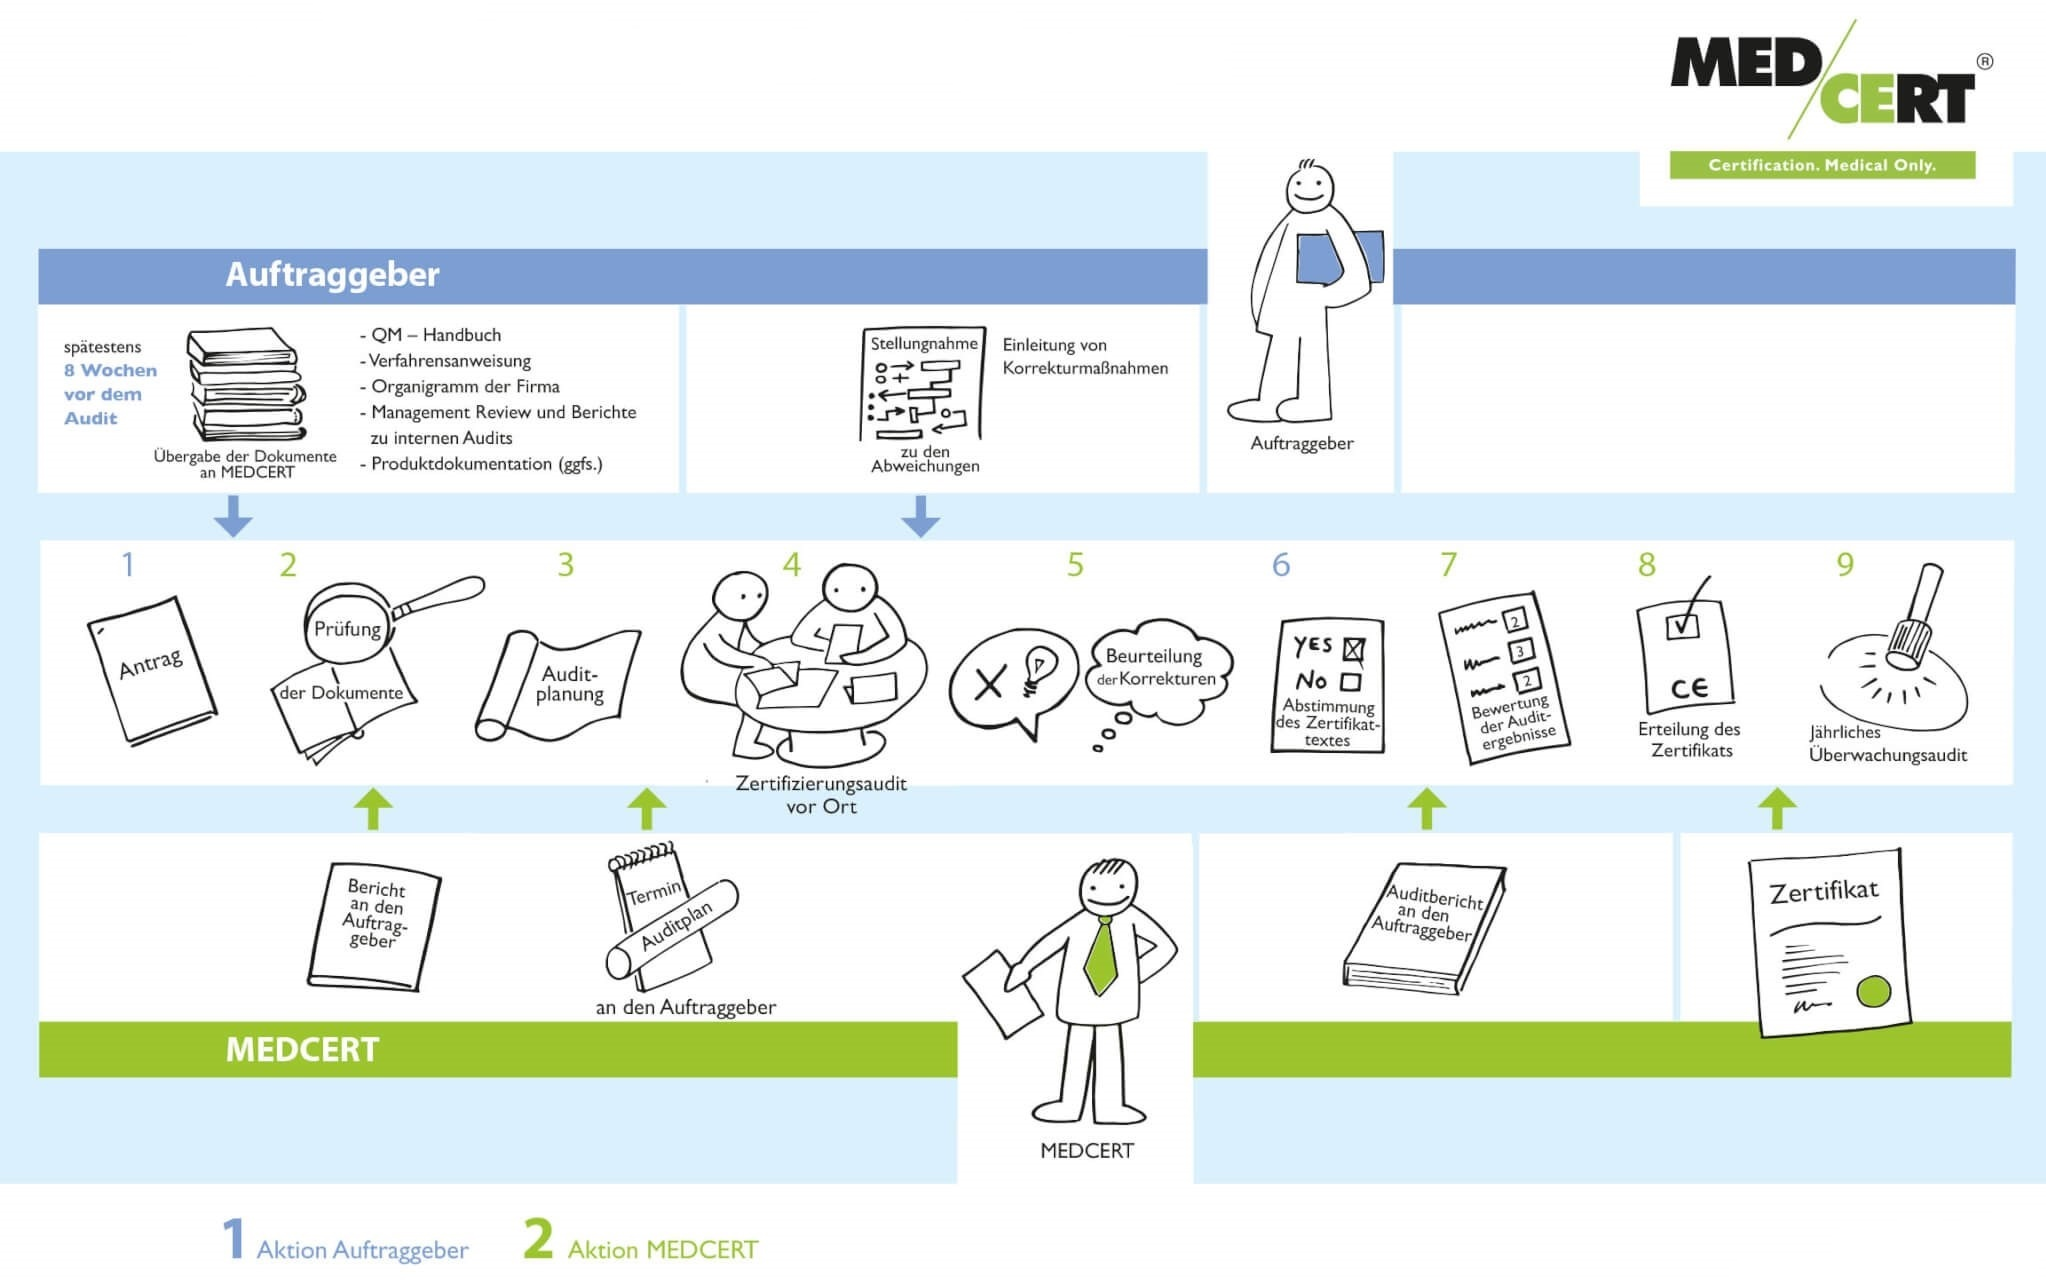
\includegraphics[width=1.0\textwidth]{images/Zertifizierungsablauf.jpg}
    \caption{\label{fig:Zertifizierungsablauf}
        Ablauf des Zertifizierungsverfahrens
        \protect\footfullcite{zertifizierungsverfahren}
    }
\end{figure}
Medizinprodukte wie Röntgengeräte, Implantate, Sehhilfen, Herzschrittmacher, 
Infusionen und Software sind Produkte, die einen bestimmten medizinischen Nutzen am Menschen haben   \cite{Marktzugangsregelung}.
Es wird nicht zwischen physikalischen Geräten mit eingebetteter Software und Geräten, die selbst die Software sind, unterschieden. 
Software als Medizinprodukt (SaMD) wird ebenfalls mit denselben Vorschriften, Richtlinien und Gesetzen entwickelt, sowie medizinische Geräte selbst \cite{AI_in_EU}.\\
Medizinprodukte werden mit der Klassifizierungsregel in vier Risikoklassen eingeteilt.
Die Regeln für die Anwendung der Klassen I, IIa, IIb und III, 
richten sich nach den Zweckbestimmungen der Produkte und liegen in der Verantwortung der Hersteller\cite{Marktzugangsregelung}. Hier werden strenge Anforderungen an die Medizinprodukthersteller gestellt. 
Medizin der Klasse I ist allerdings davon ausgeschlossen, hier reicht eine Selbsterklärung des Herstellers.\\
In Abbildung~\ref{fig:Zertifizierungsablauf} wird der Verlauf der Zertifizierung von Medizinprodukten in Deutschland von MEDCERT dargestellt.
MEDCERT ist eine Benannte Stelle und Zertifizierungsgesellschaft,
die von der Zentralstelle der Länder für Gesundheitsschutz (ZLG) zertifiziert wurde \cite{Marktzugangsregelung}.
Als ersten Schritt muss der Hersteller bei obengenannter Bennanten Stelle einen Antrag stellen. Wichtige Dokumente wie die Qualitätsmanagement-Dokumentation,
das Organigramm der Firma,
die Berichte zu internen Audits und gegebenenfalls Produktdokumentationen werden an MEDCERT übergeben.
Diese werden in Schritt zwei von der Bennanten Stelle nach den Normen und Anforderungen geprüft.
Hier wird auf die Medizinprodukteverordnung 2017/745 (MDR), die am 25. Mai 2017 in Kraft trat,
zurückgegriffen \cite{Produkteverordnung}.
Diese stellt mit drei Richtlinien  die Ansprüche an die Konformitätsbewertungen von Medizinprodukten.
In Schritt drei und vier wird ein Termin vereinbart, in dem genau beschrieben wird, welche Bereiche wann geprüft werden.
Anschließend werden in Schritt fünf und sechs die eingereichten Korrekturmaßnahmen beurteilt und der Zertifikatstext abgestimmt.
In Schritt sieben wird das gesamte Zertifizierungsverfahren bewertet.
Das erfolgreiche Durchlaufen des Verfahrens der Benannten Stelle stellt sicher,
dass das Medizinprodukt alle geltenden Anforderungen erfüllt
und die Hersteller für ihr Medizinprodukt nun die entsprechende CE-Kennzeichnung bekommen \cite{AI_in_EU}.
Schritt neun in Abbildung~\ref{fig:Zertifizierungsablauf} zeigt, dass nun ein jährliches Überwachungsaudit folgt.
Die Medizinprodukte entwickeln sich ständig weiter, werden verbessert und erneuert. 
Diese Änderungen müssen laufend von der Benannten Stelle überprüft und genehmigt werden,
sofern vorgeschriebene Anforderungen beeinträchtigt werden.
Laufende Richtlinien werden immer wieder mit neuen Verordnungen korrigiert und ergänzt.\\
Normungsgremien wie die International Organization for Standardization (ISO) und die International Electrotechnical Commission (IEC) sowie europäische Normungsorganisationen bekräftigen europäische Normen, die im Folgenden erklärt werden. 
Die europäische Normen beinhalten die benötigten rechtlichen Anforderungen für die jeweiligen medizinischen Produkte. Den Herstellern steht es frei, sich an den Normen zu orientieren. Jedoch kann durch Einhaltung der Normen die Konformität nachgewiesen werden \cite{AI_in_EU}.
Einige ISO und IEC Normen treffen auf die regulierenden Anforderungen zu.
So werden die Qualitätsanforderungen für die Entwicklung von Medizinprodukten weitestgehend durch die harmonisierte Norm ISO 13485 bestimmt \cite{iso13485}. 
Um für die Sicherheit der Menschen bei klinischer Prüfung von Medizinprodukten zu sorgen, dient die Norm ISO 14155  \cite{iso14155}.
Die Norm ISO 14971 ist für den Risikomanagementprozess von Medizinprodukten verantwortlich \cite{iso14971}.
Außerdem folgende drei IEC Normen.
Der Software Lebenszyklus von Medizinprodukten fällt unter die Norm IEC 62304 \cite{iec62304}. 
Anwendung der Gebrauchstauglichkeit, durch Entwicklungsprozesse,
auf Medizinprodukte lässt sich auf die Norm IEC 62366-1 zurückführen \cite{iec623661}. 
Die Norm IEC 82304-1 beschäftigt sich mit allgemeinen Anforderungen für die Produktsicherheit \cite{iec823041}.
			\subsubsection{Medizinische Geräte mit Künstlicher Intelligenz}\label{sec:europe-with-ai}
				Künstliche Intelligenz (KI) ist ein Teilgebiet der Informatik. Automatisierung von intelligentem Verhalten und maschinelles Lernen (ML) stehen im Vordergrund. Mit dem Einsatz von KI und ML können laufend neue Erkenntnisse gewonnen werden.
Diese sind nützlich, um brauchbare Systeme für Patienten zu entwickeln.\cite{AI_in_EU}\\
In Kapitel~\ref{sec:ki-today} wird auf die Verwendung der Medizinprodukte mit KI eingegangen.
Der Unterschied zwischen Software als Medizinprodukt (SaMD) und Künstlicher Intelligenz mit maschinellen Lerntechnologien liegt darin, dass letzteres die Fähigkeit besitzt, 
Geräteleistungen in Echtzeit anzupassen und zu optimieren.\cite{AI_in_EU}\\
So kann die Gesundheitsversorgung der Patienten durchgehend verbessert werden. 
Obwohl sich die Medizinprodukteverordnung (MDR) nicht ausdrücklich mit medizinischen KI\-Systemen befasst, 
liegt es nahe, dass dieselben Richtlinien auch für KI-Systeme gelten. 
Bei Gesetzen und Normen für medizinische Produkte mit KI wird sich ebenfalls stark an die US\-amerikanische Food and Drug Administration (FDA) gelehnt. 
Dennoch gibt es Unsicherheiten, wie mit solchen Systemen im weiteren Verlauf umgegangen werden soll.\footfullcite{fda} Rahmenbedingungen, die es schon teilweise gibt, sollen den laufenden Entwicklungen angepasst werden.
		\subsection{Zulassungsverfahren in den Vereinigten Staaten von Amerika \small{(Alex)}}\label{sec:us}
			Zentrale Fragestellung
			\subsubsection{Medizinische Geräte ohne Künstliche Intelligenz}\label{sec:us-no-ai}
				Die Zulassung von Medizinischen Produkten jeglicher Art fällt unter die Verantwortung der FDA, der Lebensmittelüberwachungs- und Arzneimittelbehörde  der Vereinigten Staaten. Sie entscheiden über die Zulassung von Medikamenten, Lebensmitteln und Medizinischen Geräten sowie auch Medizinischer Software. Autorität zur Überwachung des Marketings und Verkaufs von Pharmazie Produkten oder Medizinischen Produkten bekam die FDA 1938 mit dem "`Federal Food, Drug, and Cosmetic Act"'. Damit war die legislative Basis gegeben. Im Jahr 1970 wurden neue Standards und Einteilungen für Medizinische Geräte präsentiert, da in den Jahren davor sich legislative Lücken gezeigt haben und der Verbraucherschutz nicht gegeben war. Unter anderem war eine Einteilung der Medizinischen Geräte in drei Klassen vorgesehen. Die Klasse I besteht aus Medizinische Produkte ohne ein besonderes Risiko. Die Sicherheit kann mit allgemeinen Kontrollen gewährleistet werden wie bestimmten Produktionsstandards und korrekter Beschriftung.\footfullcite{fdagc} Die Klasse II Produkte haben ein gemäßigtes Risiko und müssen bestimmte Performance Charakteristiken erfüllen um zugelassen zu werden. Dazu werden sie jeweils mit einem vergleichbaren Produkt verglichen um die Sicherheit zu gewährleisten. Außerdem werden sie nach Einführung strenger überwacht und müssen ebenfalls korrekt Beschriftet werden. Klasse III sind die Produkte mit dem höchstem Risiko und müssen vor Markteinführung kontrolliert und in klinischen Tests getestet werden. Außerdem gilt, wenn es für ein Klasse II Produkt kein vergleichbares Produkt gibt, muss es denn gleichen Prozess durchlaufen wie Produkte der Klasse III.\footfullcite{fdacls} Im Jahr 1976 wurden diese Empfehlungen dann umgesetzt. Damit ergibt sich aber das Problem das Klasse II Geräte mit niedrigem Risiko trotzdem die langwierigen Verfahren von Klasse III Produkten durchlaufen müssen. Um das Problem zu lösen wurde der "`De Novo"'\cite{usa_ai_approval} weg zur Zulassung erstellt. Für Geräte mit niedrigem Risiko welche aber keine vergleichbaren Produkte haben. Außerdem gibt es auch für Klasse III Produkte ein beschleunigtes Verfahren wenn es das Potenzial hat Menschen mit schweren und seltenen Krankheiten zu helfen. Die Klasse von Medizinischen Geräten wird bestimmt indem die Datenbank der FDA nach dem Produkttyp durchsucht wird.\footfullcite{fdamdc} Software wird anders gehandhabt. Sie wird nach dem Benutzungsziel klassifiziert. Dabei gibt es vier Klassen mit steigendem Risiko. Klasse I und II beschreibt Software welche nur zur Verwaltung oder zum Informieren des Personals gedacht ist. Klasse II und III sind Klassen für Software welche für kritische Verwaltende Aufgaben genutzt wird oder zur Behandlung und zum Diagnostizieren von Krankheiten verwendet wird. Dabei die höchste Klasse IV für Kritische Einsatzfelder beim Behandeln oder Diagnostizieren reserviert ist. Es gibt noch die Besonderheit das Software, welche ein Gerät steuert nicht in die Software-Klassen eingeteilt wird sondern wie ein normales Gerät behandelt wird. \cite{usa_ai_approval}
			\subsubsection{Medizinische Geräte mit Künstlicher Intelligenz}\label{sec:us-with-ai}
				Zentrale Fragestellung

	\newpage
	\section{Kriterien für die Zulassung von medizinischen Produkten mit KI}\label{sec:analysis}
				\input{partials/special-criteria}
			\subsection{Verwendung medizinischer Produkte mit KI in der heutigen Medizin \small{(Miriam)}}\label{sec:ki-today}
				Die Künstliche Intelligenz erlebte seit ihrer Geburtsstunde in den 1940er und 1950er Jahren viele Rückschläge und Erfolge \cite{Chapter_14}. Im Jahr 2011 wurde das maschinelle Lernen (ML) entdeckt, was zu einem exponentiellen Entwicklungswachstum der KI führte  \cite{Chapter_14}. Besonders in der Medizin werden die Fähigkeiten künstlich intelligenter Systeme geschätzt.Dabei wird die KI im Gesundheitssystem am häufigsten für die Unterstützung bei der Diagnose, im Management und für die Erhaltung einer gesunden Lebensweise eingesetzt \cite{Opportunities_challenges_ai_hc}.\\
Weil die KI große Datenmengen verarbeiten, vergleichen und analysieren kann, wird das medizinische Personal entlastet. Menschen können zwar Muster in Daten erkennen, jedoch ist dies ein mühsamer Prozess. Ärzte übersehen infolge von Überlastung und Zeitmangel sehr leicht Anzeichen, was die Diagnose in eine falsche Richtung lenkt \cite{Opportunities_challenges_ai_hc}. Die KI kann helfen, indem sie Signale offenlegt, die sonst nicht erkannt werden \cite{Opportunities_challenges_ai_hc}.\\
Die Relevanz von KI im Gesundheitswesen wird auch durch die Tatsache belegt, dass große Unternehmen wie IBM und Google auf diesem Gebiet entwickeln. IBM Watson bietet ein Frage-Antwort-System für das Gesundheitswesen an. Es nutzt Sprache, Hypothesenbildung und evidenzbasiertes Lernen, um das medizinische Personal bei seinen Entscheidungen zu unterstützen \cite{Opportunities_challenges_ai_hc}. Ein Google Unternehmen eröffnete 2016 eine DeepMind Health Abteilung, welche u.a. auf dem Gebiet der KI Medizin arbeitet. Diese entwickelt eine ähnliche Anwendung wie IBM Watson. Die Anwendungen gibt medizinischem Personal im Einsatz Ratschläge und erkennt Veranlagungen für Krankheiten bei den Patienten  \cite{Opportunities_challenges_ai_hc}.\\
Medizinische KI Anwendungen adressieren nicht nur Ärzte, sondern auch das Management von Unternehmen im Gesundheitswesen \cite{Opportunities_challenges_ai_hc}. Quentus, gegründet 2012 in den USA, optimiert Entscheidungen in Krankenhäusern in Echtzeit um Kosten zu senken, Qualität zu verbessern und Erfahrung zu sammeln. Ziel der Anwendung ist, die Abläufe in einem Krankenhaus zu optimieren und zu vereinfachen, damit sich das medizinische Personal auf die Patientenversorgung konzentrieren kann. Quentus entwickelt als Plattform, löst die betrieblichen Herausforderungen im gesamten Krankenhaus einschließlich Notaufnahme, perioperative Bereiche und Patientensicherheit. Diese Anwendung ermöglicht somit die Integration eines Krankenhauses in ein Gesundheitssystem \cite{Opportunities_challenges_ai_hc}.\\
Immer häufiger wird KI in Programmen eingesetzt, die eine gesunden Lebensweise unterstützen sollen. Wearables, auf denen solche Programme laufen, können über ihre Sensoren auch Patientendaten sammeln \cite{Opportunities_challenges_ai_hc}.  Durch die stetige Generierung dieser Daten sind Informationen wie Vitalwerte oder Einhaltung einer Medikation bereits vor der Ankunft eines Patienten im Krankenhaus bekannt. KI Anwendungen sind in der Lage, alle diese Daten zu erfassen und zu verarbeiten. So können Leistungserbringer im Gesundheitswesen Engpässe identifizieren, um Wartezeiten der Patienten zu verkürzen, oder durch die Vermeidung unnötiger Tests Kosten senken \cite{Chapter_14}.\\


 
			\subsection{Vorteile von KI für den Patienten \small{(Miriam)}}\label{sec:ki-advantages}
				In den letzten Jahren ist die Beliebtheit der Telemedizin stark gestiegen. Einige Telemedizin-Anwendungen sammeln Informationen von tragbaren Sensoren auf Fitnesstrackern \cite{Opportunities_challenges_ai_hc}. Diese Geräte werden meistens am Handgelenk getragen und versprechen die Optimierung von Wohlbefinden und Gesundheitszustand in der modernen, von Stress geplagten Gesellschaft. Ein Benutzer/Benutzerin kann beispielsweise seinen Schlafrhythmus analysieren oder seine Fitnesszustand anhand von Parametern wie Herzfrequenz oder verbrauchten Kalorien ständig überwachen \cite{Opportunities_challenges_ai_hc}. \\
Andere Softwareanwendungen interagieren mit dem Patienten, um eine Verdachtsdiagnose zu stellen  \cite{Opportunities_challenges_ai_hc}. Sie stellen den Nutzer Fragen über eine vermutete Erkrankung oder ein gesundheitliches Problem und nutzen Spracherkennung oder Texterkennung, um ihm eine mündliche oder schriftliche Antwort zu ermöglichen.
Zu den beliebtesten Anwendungen dieser Art gehören ADA und Your.MG. Die Gesundheitshilfe ADA wurde von einem deutschen Startup Unternehmen entwickelt und weltweit in über 130 Länder (Stand 2016) eingeführt \cite{Opportunities_challenges_ai_hc}. ADA kann kostenlos auf alle Mobilgeräte geladen werden. Nach Installation und Anmeldung gibt der Nutzer seine Beschwerden und Symptome in einen Textdialog ein und bekommt Erläuterungen und Ratschläge, was er aufgrund seiner Symptome als nächstes unternehmen soll.\\
Eine weiter Anwendung von KI ist Telehomecare, eine Alternative zum traditionellen Krankenhausaufenthalt \cite{Chapter_14}. Die häusliche Pflege ist einer der am schnellsten wachsenden Märkte der Welt \cite{Chapter_14}. Hier geht es um Patienten, die postoperativ nach einem Krankenhausaufenthalt oder aufgrund von Alter oder Gebrechlichkeit zu Hause gepflegt werden müssen. Die häusliche Pflege hat sich bereits so weit entwickelt, dass auch Palliativpatienten zu Hause gepflegt werden können. Palliativepflege ist nach WHO die aktive um­fassen­de Pflege von Patienten, die an ei­ner nicht heil­baren, fort­schreiten­den und so weit fort­ge­schritte­nen Erkrankung leiden, dass dadurch ih­re Le­bens­er­wartung be­grenzt ist \cite{Pschyrembel}. Solche Pflege minimiert Infektionsrisiken und senkt die Kosten für die Patienten erheblich. Zudem trägt die Pflege in einer bekannten Umgebung mit intensivem Kontakt zur Familie stark zu positiven Behandlungsergebnissen bei.
Bei der Umsetzung von Telehomecare senden Warnsysteme, die sich in der Wohnung der Patienten befinden, Benachrichtigungen an ein Telemonitoring Zentrum, nachdem sie Daten über die Bedürfnisse des Patienten gesammelt haben \cite{Chapter_14}. Diese Information werden in den Telemonitoring Zentren durch ein Pfleger/Pflegerin und einen Arzt/Ärztin ausgewertet. Sie können in Echtzeit auf kritische Daten des Patienten zugreifen, um Komplikationen zu vermeiden, eine Zustandsverschlechterung des Patienten zu verhindern oder auf einen Notfall zu reagieren \cite{Chapter_14}.\\
Die starke Weiterentwicklung und das Wachstum der mobilen Technologien trägt dazu bei, dass die positiven Auswirkungen der KI gestützten häuslichen Pflege noch größer sind, wenn sie mit der Verwendung von tragbaren Geräten verbunden sind. Auch hier trägt der Patient Sensoren auf einem Armband, mit denen er in Echtzeit überwacht wird. Im Fall einer psychischen Krankheit hat die Familie die Möglichkeit, den Aufenthaltsort des Betroffenen zu überwachen \cite{Chapter_14}.
			\subsection{Grenzen von KI in der Medizin  \small{(Miriam)}}\label{sec:ki-limitations}
				Trotz der großen Menge an Vorteilen, welche die KI Technologien im Gesundheitssystem mitbringen, sind die Herausforderungen für die weitere Etablierung mindestens genau so groß. Für das ordnungsgemäße Funktionieren von Softwareanwendungen, in denen KI Techniken zum Einsatz kommen - im folgenden als 'KI-Systeme' bezeichnet - ist wesentlich, dass die Leistungserbringer im Gesundheitssystem die Daten, die zur Schulung dieser Anwendungen verwendet werden, auswerten, um das Einschleichen von Verzerrungen zu verhindern \cite{Chapter_14}. In der Diagnostik können solche Verzerrungen zu falschen Befunden führen.\\
Die Überanpassung von Algorithmen ist eine der Ursachen, die die Anwendung der KI in der Medizin eingrenzen. Von einer Überanpassung spricht man, wenn KI Algorithmen, die auf einen bestimmten Datensatz trainiert wurden, nur begrenzt auf andere Datensätze anwendbar sind \cite{AI_where_are_we_now}. Der KI Algorithmus hat dann ausschließlich die statischen Variationen der Trainingsdaten gelernt, anstatt der allgemeinen, zur Problemlösung notwendigen Konzepte. Die Überanpassung eines Algorithmus wird von mehreren Faktoren beeinflusst wie der Größe des Datensatzes, dem Ausmaß der Heterogenität\footfullcite{heterogen} der Daten und der Verteilung der Daten innerhalb des Datensatzes. Ein Modell kann überangepasst sein, wenn sich die Krankheitshäufigkeit und die Anzahl der neu auftretenden Krankheitsfälle zwischen den Trainings- und Testsätzen erheblich unterscheiden \cite{AI_where_are_we_now}. Überanpassung kann aber auch auftreten, wenn die Trainings- und Testsätze mit wesentlich unterschiedlichen Parametern oder Geräten erzielt wurden \cite{AI_where_are_we_now}.\\
Einer der größten Kritikpunkte an der Integration von KI in der Medizin ist, dass sich KI-Systeme von außen betrachtet wie eine Black-Box verhalten \cite{The_missing_pieces}. Gemeint ist, dass es nicht möglich ist, nachzuvollziehen, wie Deep Learning Algorithmen zu ihrer Entscheidung gekommen sind \cite{The_missing_pieces}. Zum Beispiel kann ein Arzt, der von einem KI-System einen radiologischen Befund gemeldet bekommt, weder sagen, welche Verfahrensmerkmale für die Analyse verwendet wurden, noch wie sie analysiert wurden und warum der Algorithmus zu diesem Ergebnis kam\cite{The_missing_pieces}. Der Mangel an Transparenz hat deshalb die KI in der wissenschaftlichen Gemeinschaft bisher zurückgedrängt, denn oft ist das „Warum“ hinter einer Vorhersage genauso wichtig wie die Vorhersage selbst \cite{The_missing_pieces}.\\
Weitere Problemfelder für die KI im Gesundheitswesen sind Privatsphäre und Informationssicherheit \cite{Opportunities_challenges_ai_hc}. In jedem Bereich unserer Gesellschaft ist die IT-Sicherheit inzwischen ein wichtiges Thema geworden. Im Gesundheitswesen wird dies besonders kritisch gesehen, weil Softwareanwendungen unmittelbar mit Menschenleben verbunden sind und ein Cyberangriff im ungünstigsten Fall sogar zum Tod von Patienten führen kann \cite{Opportunities_challenges_ai_hc}.\\
Auf dieser Grundlage stellen sich eine Reihe von weiteren Fragen: Welcher Schutz gilt als zuverlässig? Wer bewertet die Zuverlässigkeit? Und nicht zu vergessen: Wer trägt die Verantwortung? 
Die Frage der Verantwortlichkeit wird gerade in einem konkreten Fall diskutiert: bis heute wurde die Roboterchirurgie mit 144 Todesfällen in den Vereinigten Staaten in Verbindung gebracht \cite{Chapter_14}. Wer ist verantwortlich? Das Unternehmen, der Entwickler oder der Dienstleister \cite{Chapter_14}?

	\newpage
	\section{Diskussion}\label{sec:discussion}
		\input{partials/discussion}
		\subsection{Lösungsansätze zur Zulassung von KI  \small{(Miriam)}} \label{sec:solutions}
			Sowohl das Blackbox-Problem auch Überanpassung der Algorithmen bilden zusammen Barrieren für die Zulassung der Medizinprodukte mit KI. Die Zulassungsstellen haben Schwierigkeiten zu bestimmen, wie und ob die Algorithmen funktionieren und ob ihre Leistung auch auf andere Datensätze anwendbar sind.\cite{AI_where_are_we_now} Es wurden aber bereits Möglichkeiten entwickelt die zum einen die Black-Box der KI öffnen und zum anderen die Übereinpassung der Algorithmen mit bestimmten Methoden festgestellt oder verhindert werden können.\cite{AI_where_are_we_now} \\

Bei dem Black-Box-Problem wurde in unterschiedlichen Studien eine Heatmap erstellt, um Regionen mit erhöhten Aktivierung des tiefen Lernnetzwerks aufzuzeichnen. Man schließt daraus, dass es sich bei der stark aktivierten Bereichen um die Regionen handelt die für die Bestimmung der Diagnose entscheidend sind.\cite{AI_where_are_we_now}\\
Die Übereinpassung kann überprüft werden in dem die Algorithmen nach dem Training an mehreren verschiedenen Datensätzen getestet werden.\cite{AI_where_are_we_now} Tests werden grafisch mit einer AUC - area under the curve  dargestellt. Bei einem Algorithmus der an eine Übereinpassung leidet wurde man erwarten, dass seine Genauigkeit gemessen mit AUC, bei Datensätzen die nicht den gleichen Ursprung haben wie die Trainingsdaten, deutliche schlechter sind.\cite{AI_where_are_we_now}\\
		\subsection{Aktuelle Richtlinien für medizinische Produkte mit KI \small{(Alex)}}\label{sec:guidlines}
			KI unterstützte Medizinische Software wird wie eine gewöhnliche Software zugelassen, obwohl sie nicht wie eine gewöhnliche Software arbeitet. Tatsache ist aber auch das die Personen in den Ämtern sich dieses Problems bewusst sind und nach besten Wissen und Gewissen versuchen werden die Sicherheit zu gewährleisten. Die in Kapitel \ref{sec:europe} und Kapitel \ref{sec:us} beschriebenen Verfahren sind darauf ausgelegt Innovationen zu ermöglichen. Der amerikanische "`De Novo"' Weg, an den sich auch die Europäische Union orientiert, bietet die Möglichkeit weniger kritische KI im Feld zu testen und ermöglicht das sammeln von Erfahrung bei der Zulassung von Medizinischen Produkten mit KI. Kritische KI, welche zum Beispiel hauptverantwortlich für das Leben eines Patienten sein soll, wird immer noch mit den strengsten Kriterien und klinischen Test geprüft bevor die Markteinführung erlaubt wird. Die aktuellen Richtlinien besitzen noch keine Spezialisierung auf KI, ermöglichen aber das Nutzen von neuen Medizinischen Produkten mit KI. Je nach Einsatzgebiet werden angepasste Zulassungsverfahren gewählt. Medizinische Produkte mit KI werden genauso streng behandelt wie Medizinische Produkte ohne KI welche das selbe Risikoniveau haben.
		\subsection{Evaluation der Zulassungskriterien für medizinische Produkte mit KI \small{(Evelyn)}}\label{sec:sufficient-criteria}
			Wie in Kapitel~\ref{sec:europe-with-ai} und Kapitel~\ref{sec:us-with-ai} zu sehen,
gibt es noch kein spezielles/spezifisches Gesetz für die Verwendung von Medizinprodukten mit KI.
Die Zulassungsverfahren von Medizinprodukten ohne KI werden bislang für die Zulassung von Medizinprodukten mit KI angewendet.
Für den Einsatz von Medizinprodukten mit KI, in kritischen Bereichen, müssen die Richtlinien angepasst und ergänzt werden.
Daraus entstehen neue Herausforderungen, die zu bewältigen sind.
Kapitel~\ref{sec:europe-with-ai} zeigt außerdem, dass von der EU-Kommission weitere Anforderungen aufgestellt werden.
In den USA werden ebenso zusätzliche Richtlinien aufgestellt.
Themen, wie ethische und rechtliche Regelungen sowie einige Fragen bleiben allerdings noch offen.
Werden die Daten der Patienten richtig verwendet? Kann die KI voreingenommen sein?
Werden Arbeitsplätze der Ärzte gestrichen? 
Wird die Versorgung auf Grund der KI besser oder schlechter? 
Mit gut durchdachten und klar definierten Regeln für die Verwendung von Medizinprodukten mit KI könnten einige
der aufkommenden Fragen und Bedenken geklärt werden.\\
Des Weiteren soll die Transparenz verbessert und exakte Qualitätsanforderungen aufgestellt werden.
Die oben genannten neuen Anforderungen und die Antworten auf die gestellten Fragen sind wichtig, 
um die Zulassungsverfahren für die Verwendung von Medizinprodukten mit KI zu erweitern,
auszubauen und präziser zu spezifizieren.
		
	
	\newpage
	\section{Fazit \small{(Miriam)}}\label{sec:conclusion}
		\input{partials/conclusion}
		\subsection{Zusammenfassung der Ergebnisse}\label{sec:summary}
			Abschließend kann man sagen, dass sich die Zulassung von Medizinprodukten mit KI stark an die Zulassung von Medizinprodukten ohne KI anlehnt. Dies bedeutet jedoch keinesfalls einen reibungslosen Verlauf des Zulassungsverfahren. 
Bei der Zulassung medizinischer Produkte mit KI gestützter Software bestehen Probleme durch mangelnde Vergleichbarkeit der Produkte, fehlende Transparenz oder Überanpassung von KI Algorithmen, undefinierten Verantwortlichkeiten und dem Fehlen von ethischen und rechtlichen Prüfungen. Dies lässt die Zulassungsverfahren langwierig und kostspielig werden.
Für einige dieser Probleme existieren bereits Lösungen. So kann dem Black-Box Problem durch grafische Darstellung diagnoserelevanter Regionen innerhalb des Neuronalen Netzes, dem Problem der Überanpassung durch Vergleiche mit Daten unterschiedlicher Herkunft entgegengewirkt werden.\\ 
Da bisher nur wenige Produkte mit KI auf dem Markt sind, werden, mangels Vergleichbarkeit, Medizinprodukte der Klasse II in die Risikoklasse III eingestuft. Damit diese Zulassungsverfahren nicht mit aufwändigen klinischen Test verbunden sind, gibt es in den USA das beschleunigte De Novo Zulassungsverfahren.\\
Auf die Entwicklung von KI Systemen für die Medizin reagiert auch die europäische Gesetzgebung. Die EU-Kommission stellt zusätzliche Anforderungen an Transparenz, Robustheit und Sicherheit von Medizinprodukten mit KI. Dies führt jedoch nicht zwangsläufig zur Vereinfachung des Zulassungsverfahren. 
Es steht fest, dass aufgrund der noch offenen Fragen der  Verantwortlichkeiten und dem Fehlen von ethischen und rechtlichen Prüfungen die Zulassungsverfahren um weitere spezifische Kriterien ergänzt werden müssen. 
Es bleibt abzuwarten, ob weitere Maßnahmen seitens der Gesetzgebung einen positiven Einfluss auf die Machbarkeit der Zulassungsverfahren bewirken.



		\subsection{Bewertung der Ergebnisse}\label{sec:rating}
			\input{partials/rating}
		\subsection{Ausblick}\label{sec:perspective}
			Die KI ist aus dem Gesundheitssystem nicht mehr wegzudenken. Die Interaktion des Menschen und KI bleibt im Vordergrund und fordert zwangsläufig die perfekte Mensch-Computer-Symbiose. Sie gibt uns den Anstoß, ein KI - System zu entwickeln, welches intelligente Fragen stellt, anstatt zu versuchen, den Arzt zu ersetzen. Außerdem unterstützen Transparenz und Zuverlässigkeit der KI Algorithmen den Einzug in die Medizin. Zum anderen müssen die Fragen der Verantwortlichkeit und Privatsphäre im Gesundheitswesen weiter ausgearbeitet werden. Wenn alle diese Punkte gelöst werden können wird die KI als ein großartiges Instrument zur Rettung von Leben und zur Verbesserung der Lebensqualität jeden Tag dienen können.
	  

    \newpage
    \printglossary[type=\acronymtype,title={Akronyme}]
   
    \newpage
    %\section*{Literatur}
    %\addcontentsline{toc}{section}{Literatur}
    \nocite{*}
    \printbibliography{}
	
    \newpage
    \printglossary[type=main,title={Glossar}]

\end{document}
